\documentclass[]{article}
\usepackage{booktabs}
\usepackage{graphicx}  % graphics
\usepackage{float} % floats
\usepackage{siunitx}
\graphicspath{{../img/}}

\newcommand{\eVal}{$1.602 * 10^{-19} \si{\coulomb}$}
\newcommand{\hVal}{ $6.626 * 10^{-34}\si{\joule\second}$ }
\newcommand{\yellowFreq}{$5.19 * 10^{14}$}
\newcommand{\greenFreq}{$5.49 * 10^{14}$}
\newcommand{\he}{$(4.20 \pm 0.03) * 10^{-15} \si{\joule\second\per\coulomb}$}
\newcommand{\hMeasured}{$(6.73 \pm 0.04) * 10^{-34} \si{\joule\second}$}
\newcommand{\we}{$1.45 \pm 0.02 \si{\joule\per\coulomb}$}
\newcommand{\wMeasured}{$2.32 \pm 0.02 \si{\joule}$}

\title{ENPHYS253 \\ Lab 4: h/e and the Photoelectric Effect}
\author{Viraj Bangari \\ 10186046}
\date{\today}

\begin{document} 
\maketitle

\section{Introduction}
In 1921, Albert Einstein won the Nobel prize in Physics for his work in
describing the photoelectric effect~\cite{ref:nobel} as it was significant in
paving the way of modern day physics. Einstein's work was built on the efforts
of Max Planck, who determined that the energy of a photon was proportional to
its frequency. However, physics as it were known at the time predicted that the
energy of light was proportional to its intensity. By using the photoelectric
effect, Einstein was able to show that the older models of light were incorrect
and provided validity to the newer field of quantum mechanics.

Photoelectric emission occurs when light hits a material that causes an electric
current. Einstein said that energy of a photoelectron was equal to the energy of
a photon by the equation: \begin{equation}\label{eq:einstein} 
    E  = KE_{\max} + W_{0} = h\upsilon 
\end{equation} where $KE_{\max}$ is the kinetic energy of an
electron, $W_{0}$ is the work function (the minimum energy to separate an
electron from a material), $h$ is Planck's constant and $\upsilon$ is the
frequency of light. It is the purpose of this experiment to show that the energy
of a photon is independent of the intensity of light by measuring the time it
takes for beam of light to reach its stopping potential but that the energy of a
photon is dependent on its frequency by measuring Einstein's linear relationship
between stopping potential, frequency and Planck's constant.

\section{Results and Analysis}
The stopping potential data from table~\ref{tab:green} and
table~\ref{tab:yellow} were plotted into figure~\ref{fig:exponential}.  Since
the data exponentially decays, equation~\ref{eq:transmission_linear} was used to
create a linear relationship between transmission percentage and time.  This
data was plotted onto figure~\ref{fig:linear}, with the randomly distributed
residual plots on figures~\ref{fig:residgreen} and~\ref{fig:residyellow}
indicating a good linear fit for the data. The linear model supports the quantum
model prediction that increased intensity would increase the photoelectric current.
The data in figure~\ref{fig:linear} shows that the greater intensity, the less
time it takes to reach the stopping potential. The quantum model predicts that
the energy of a photoelectron is independent of the intensity of light, which is shown
in table~\ref{tab:green} and~\ref{tab:yellow} by the fact that the stopping
potential values stay constant within error.

The frequency and stopping potential values from table~\ref{tab:frequency} were
plotted against each other onto~\ref{fig:frequency}. Using a linear regression
with equation~\ref{eq:linear_einstein} and the accepted value of $e$=\we, the
value of $h/e$ was determined as \he, $h$ as \hMeasured, $W_0/e$ as \we\ and
$W_0$ as \wMeasured. The value of measured value of $h$ has a percentage
difference of 1.6\% from the accepted value of \hVal. The results from
figure~\ref{fig:frequency} support the quantum model that a higher frequency
results in higher energy photoelectrons.

\newpage
\begin{figure}[H]
    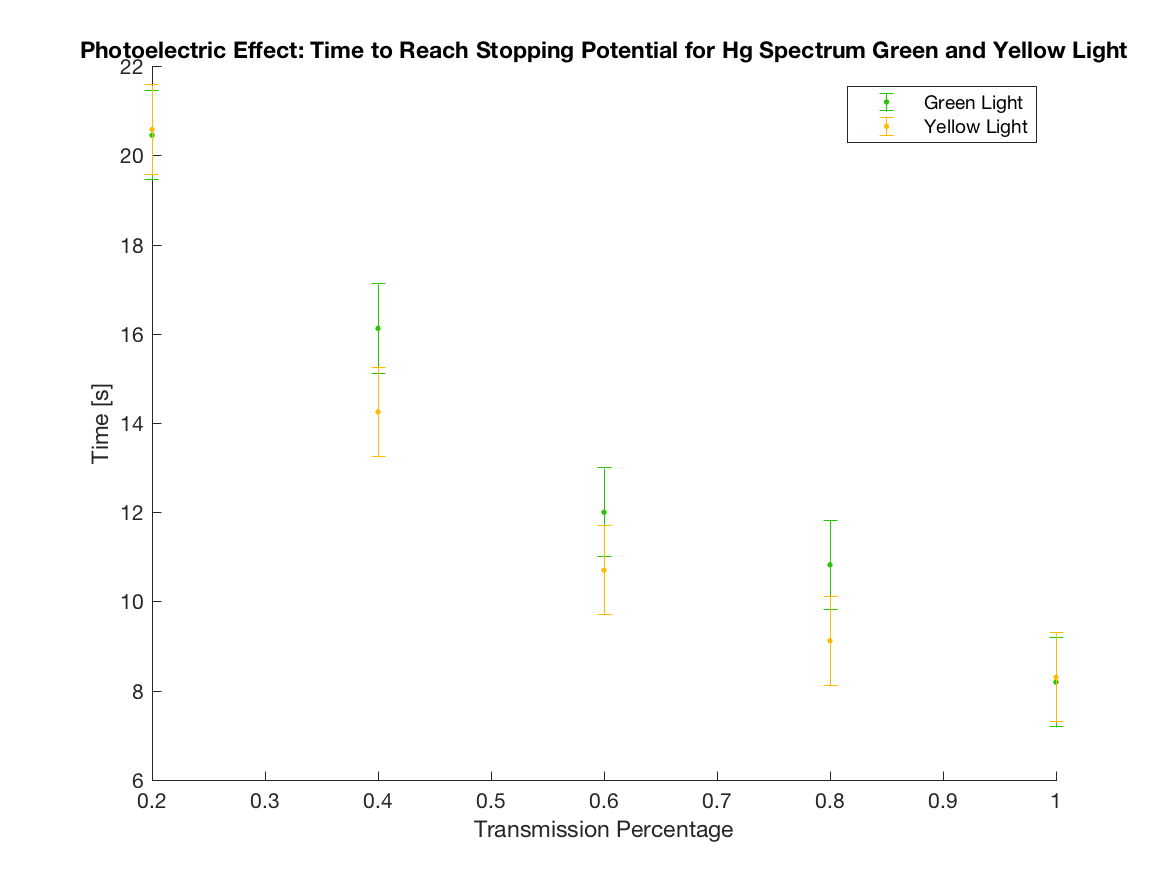
\includegraphics[width=\textwidth]{../img/exponential.png}
    \caption{Measured time to Reach Photoelectric Stopping Potential for Hg
    Spectrum Green with frequency \greenFreq\ and Yellow light with frequency
    \yellowFreq\. Note the exponential decay.
    points.}\label{fig:exponential}
\end{figure}

\newpage

\begin{figure}[H]
    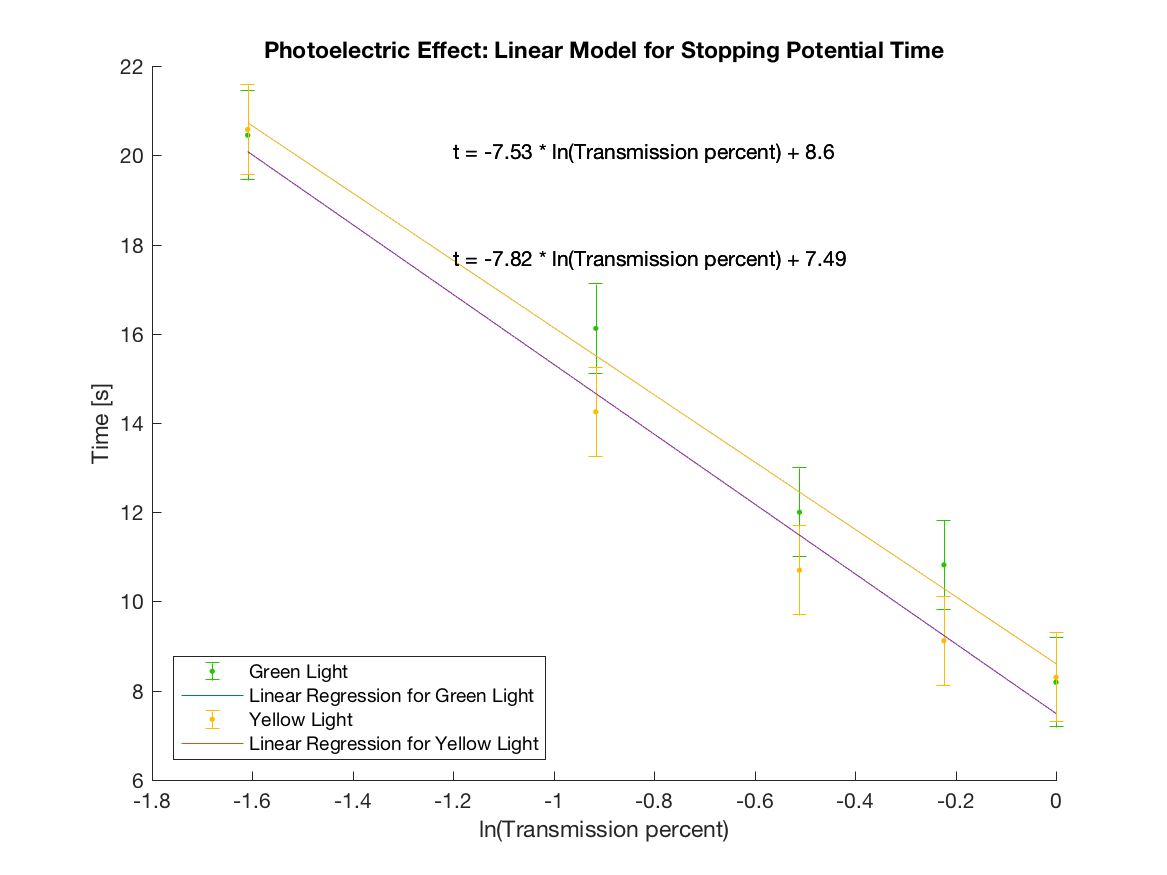
\includegraphics[width=\textwidth]{../img/linear.png}
    \caption{Linear Model for the Photoelectric Stopping Potential for Hg
    Spectrum Green with frequency \greenFreq\ and Yellow light with frequency
    \yellowFreq}\label{fig:linear}
\end{figure}
\begin{figure}[H]
    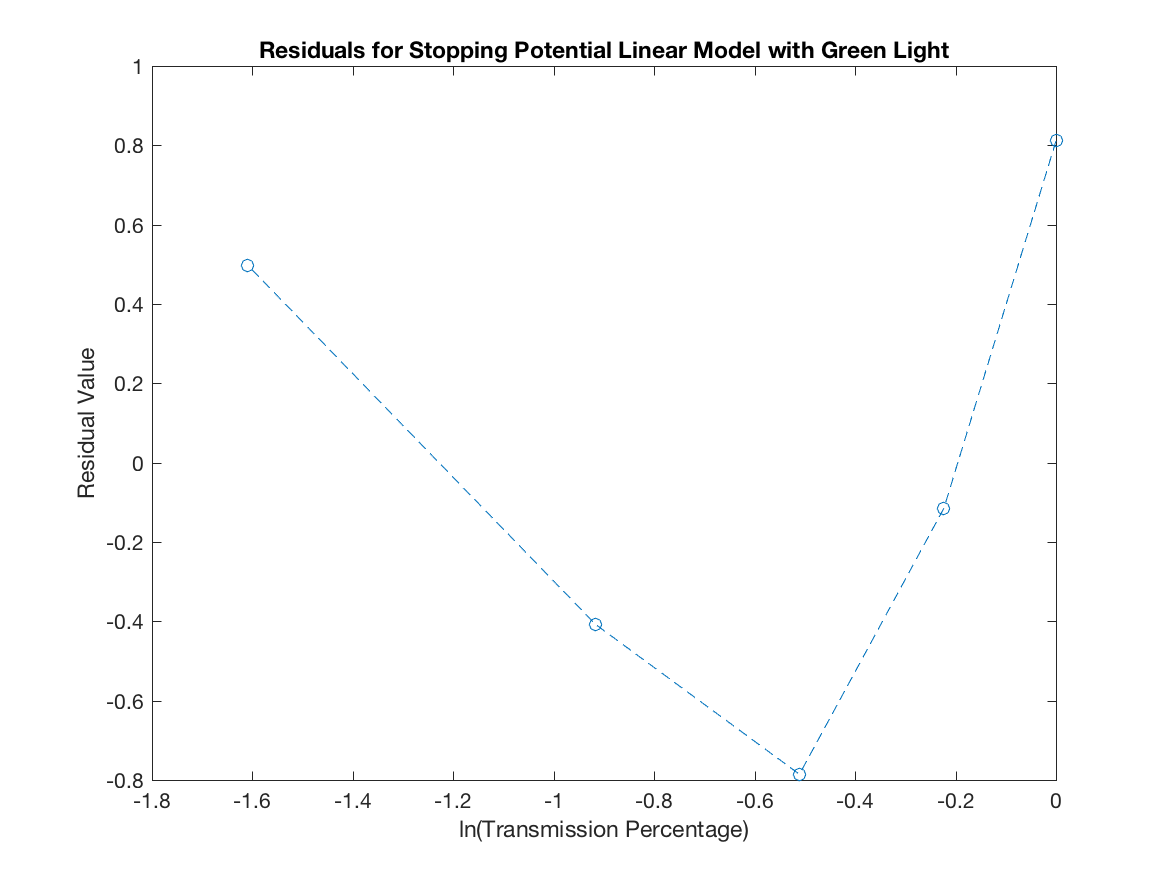
\includegraphics[width=\textwidth]{../img/residgreen.png}
    \caption{Plot of residuals for green light data
    from~\ref{fig:linear}. Note the randomness of the data.}\label{fig:residgreen}
\end{figure}
\begin{figure}[H]
    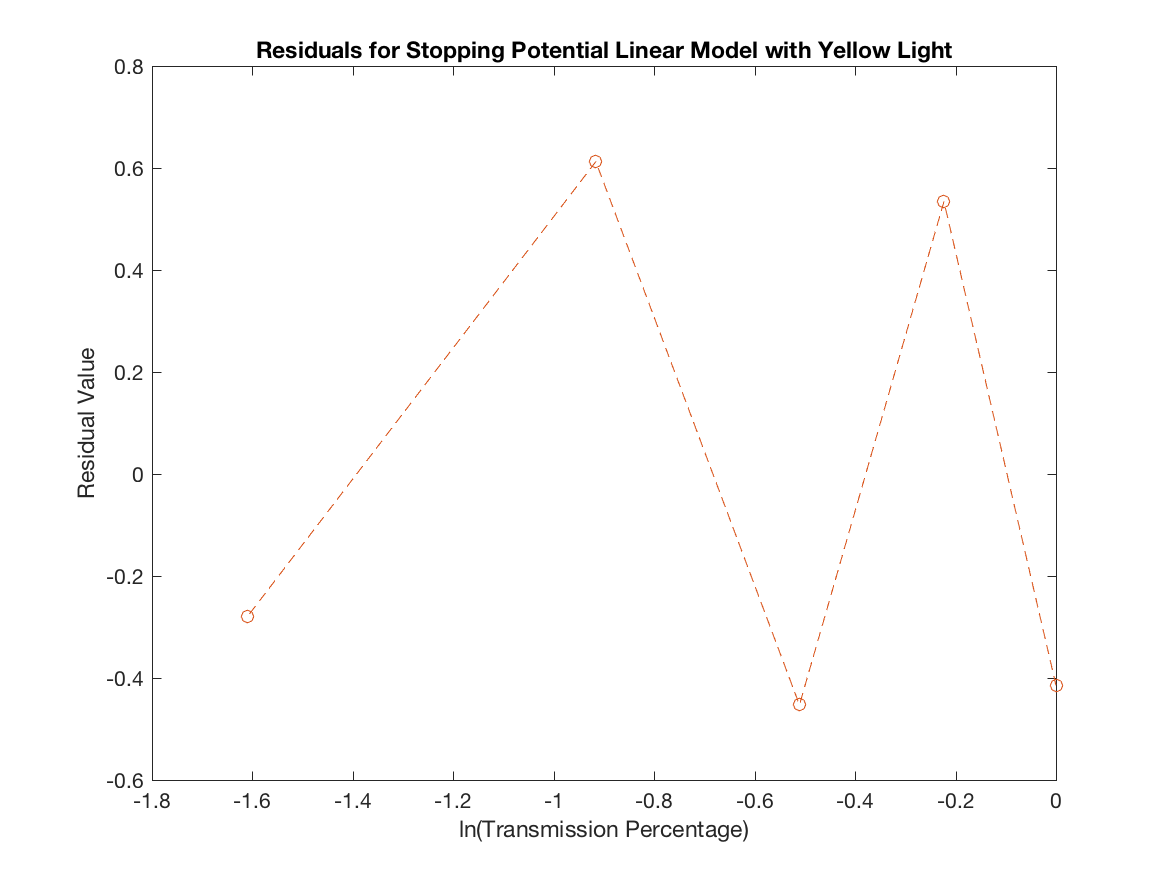
\includegraphics[width=\textwidth]{../img/residyellow.png}
    \caption{Plot of residuals for yellow light data from~\ref{fig:linear}. Note
    the randomness of the data}\label{fig:residyellow}
\end{figure}

\newpage
\begin{figure}[H]
    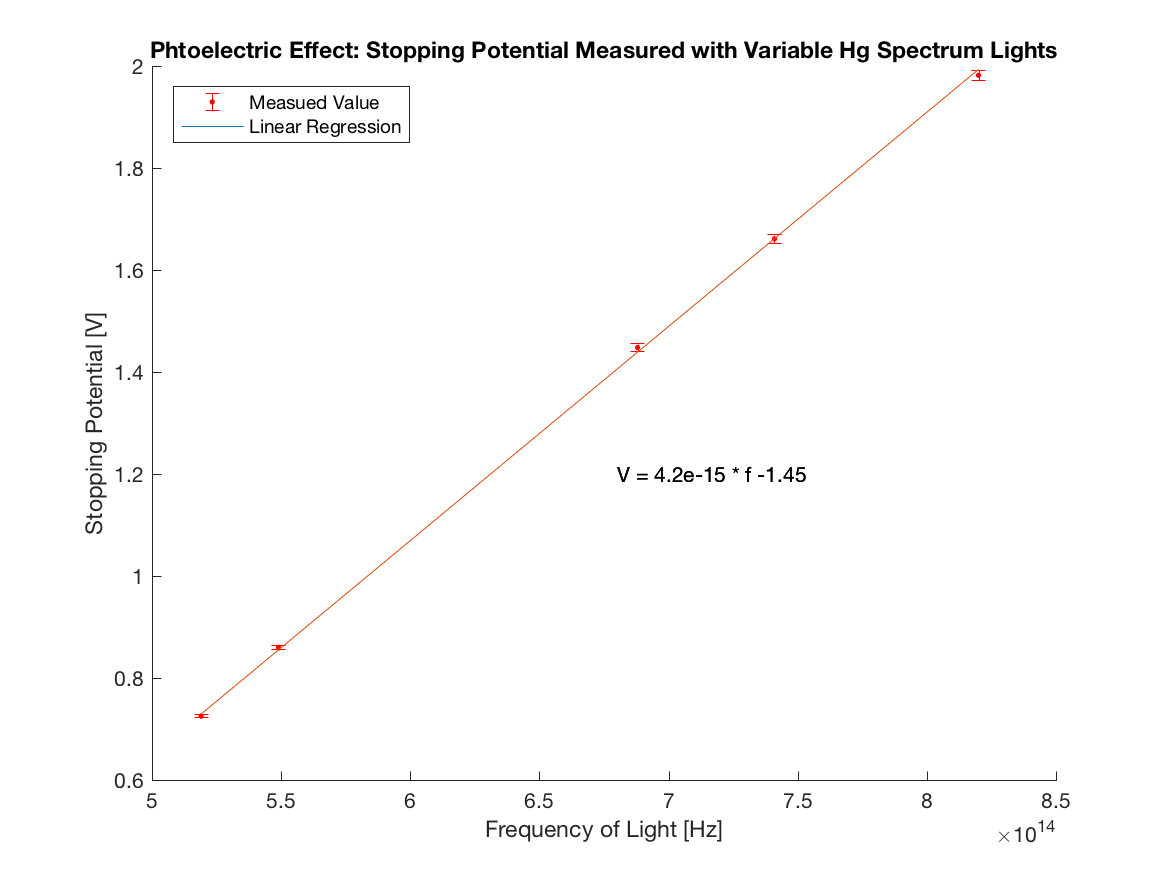
\includegraphics[width=\textwidth]{../img/stopping.png}
    \caption{Photoelectric Effect: Stopping Potential Measured with Variable Hg
    Spectrum Lights}\label{fig:frequency}
\end{figure}
\newpage

\section{Appendix}

\subsection{Equation List} 
$h$ is Planck's constant which has an accepted value of \hVal~\cite{ref:h}, $\upsilon$ is frequency, $KE_{\max}$ is the
maximum kinetic energy of the emitted photoelectrons, $W_{0}$ is the work
function, $V$ is is the stopping potential in Volts, $e$ is the charge of an
electron with an accepted value of $1.602 * 10^{-19}
\si{\coulomb}$~\cite{ref:e}, $p_{trans}$ is the transmission percentage and $t$
is the time to reach stopping potential.


\begin{equation}\label{eq:linear_einstein}
    V = (h/e)\upsilon - (W_{0}/e)
\end{equation}

\begin{equation}\label{eq:potential}
    KE_{\max} = Ve
\end{equation}

\begin{equation}\label{eq:transmission_linear}
    t = A\ln(p_{trans}) + t_{100\%}
\end{equation}

\subsection{Raw Data}

\begin{table}[H]
    \caption{Photoelectric Stopping Potential Time and Voltage for Hg Spectrum Green light
    with frequency \greenFreq$\si{\hertz}$}\label{tab:green}
    \begin{tabular}{@{}lll@{}}
        \toprule
        Transmission Percent & Stopping Potential {[}V{]} +/- 0.0042 {[}V{]} & Time to Recharge {[}s{]} +/- 1  s \\ \midrule
        100                 & 0.857                                         & 8.19                              \\
        80                  & 0.855                                         & 10.82                             \\
        60                  & 0.855                                         & 12                                \\
        40                  & 0.854                                         & 16.12                             \\
        20                  & 0.851                                         & 20.45                             \\ \bottomrule
    \end{tabular}
\end{table}

\begin{table}[H]
    \caption{Photoelectric Stopping Potential Time and Voltage for Hg Spectrum Yellow Light,
    with frequency \yellowFreq$\si{\hertz}$}\label{tab:yellow}
    \begin{tabular}{@{}lll@{}}
        \toprule
        Transmission Percent & Stopping Potential {[}V{]} +/- 0.0036 {[}V{]} & Time to Recharge {[}s{]} +/- 1  s \\ \midrule
        100                 & 0.721                                         & 8.3                               \\
        80                  & 0.720                                         & 9.12                              \\
        60                  & 0.720                                         & 10.7                              \\
        40                  & 0.719                                         & 14.25                             \\
        20                  & 0.716                                         & 20.58                             \\ \bottomrule
    \end{tabular}
\end{table}

\begin{table}[H]
    \caption{Photoelectric Stopping Potential Time for Various Hg Spectrum Lights}\label{tab:frequency}
    \begin{tabular}{@{}llll@{}}
        \toprule
        Light Colour & Frequency * $10^{14}${[}Hz{]} & Stopping Potential {[}V{]} & Error in Stopping Potential {[}V{]} \\ \midrule
        Yellow       & 5.19                          & 0.725                      & 0.0036                              \\
        Green        & 5.49                          & 0.860                      & 0.0043                              \\
        Blue         & 6.88                          & 1.448                      & 0.0072                              \\
        Violet One   & 7.41                          & 1.661                      & 0.0083                              \\
        Violet Two   & 8.2                           & 1.982                      & 0.0099                              \\ \bottomrule
    \end{tabular}
\end{table}

\subsection{Sample Calculations using Linear Regression Data
from~\ref{fig:linear}}
$h = h/e * e =$ \he\ $*$\eVal$ =$ \hMeasured\
$W_0 = W_0/e * e =$ \we\ $*$\eVal$ =$ \wMeasured\

\bibliographystyle{ieeetr}%Used BibTeX style is unsrt
\bibliography{lab4}

\end{document}
